%%%%%%%%%%%%%%%%%%%%%%%%%%%%%%%%%%%%%%%%%
% baposter Landscape Poster
% LaTeX Template
% Version 1.0 (11/06/13)
%
% baposter Class Created by:
% Brian Amberg (baposter@brian-amberg.de)
%
% This template has been downloaded from:
% http://www.LaTeXTemplates.com
%
% License:
% CC BY-NC-SA 3.0 (http://creativecommons.org/licenses/by-nc-sa/3.0/)
%
%%%%%%%%%%%%%%%%%%%%%%%%%%%%%%%%%%%%%%%%%

%-----------------------------------------------------------6-----------------------------
%	PACKAGES AND OTHER DOCUMENT CONFIGURATIONS
%----------------------------------------------------------------------------------------

\documentclass[landscape,a0paper,fontscale=0.255]{baposter} % Adjust the font scale/size here

\usepackage{graphicx} % Required for including images
\graphicspath{{figures/}} % Directory in which figures are stored

\usepackage{amsmath} % For typesetting math
\usepackage{amssymb} % Adds new symbols to be used in math mode

\usepackage{booktabs} % Top and bottom rules for tables
\usepackage{enumitem} % Used to reduce itemize/enumerate spacing
\usepackage{palatino} % Use the Palatino font
\usepackage[font=small,labelfont=bf]{caption} % Required for specifying captions to tables and figures

\usepackage{multicol} % Required for multiple columns
\setlength{\columnsep}{2em} % Slightly increase the space between columns
\setlength{\columnseprule}{0mm} % No horizontal rule between columns

\usepackage{tikz} % Required for flow chart
\usetikzlibrary{shapes,arrows} % Tikz libraries required for the flow chart in the template

\newcommand{\compresslist}{ % Define a command to reduce spacing within itemize/enumerate environments, this is used right after \begin{itemize} or \begin{enumerate}
\setlength{\itemsep}{1pt}
\setlength{\parskip}{0pt}
\setlength{\parsep}{0pt}
}

\definecolor{lightblue}{rgb}{0.145,0.6666,1} % Defines the color used for content box headers

\begin{document}

\begin{poster}
{
headerborder=closed, % Adds a border around the header of content boxes
colspacing=1em, % Column spacing
bgColorOne=white, % Background color for the gradient on the left side of the poster
bgColorTwo=white, % Background color for the gradient on the right side of the poster
borderColor=lightblue, % Border color
headerColorOne=black, % Background color for the header in the content boxes (left side)
headerColorTwo=lightblue, % Background color for the header in the content boxes (right side)
headerFontColor=white, % Text color for the header text in the content boxes
boxColorOne=white, % Background color of the content boxes
textborder=roundedleft, % Format of the border around content boxes, can be: none, bars, coils, triangles, rectangle, rounded, roundedsmall, roundedright or faded
eyecatcher=true, % Set to false for ignoring the left logo in the title and move the title left
headerheight=0.1\textheight, % Height of the header
headershape=roundedright, % Specify the rounded corner in the content box headers, can be: rectangle, small-rounded, roundedright, roundedleft or rounded
headerfont=\Large\bf\textsc, % Large, bold and sans serif font in the headers of content boxes
%textfont={\setlength{\parindent}{1.5em}}, % Uncomment for paragraph indentation
linewidth=2pt % Width of the border lines around content boxes
}
%----------------------------------------------------------------------------------------
%	TITLE SECTION 
%----------------------------------------------------------------------------------------
%
{
\includegraphics[height=4em]{logo.png}} % First university/lab logo on the left
{\bf\textsc{Tiling the Unit Square}\vspace{0.5em}} % Poster title
{\textsc{\{ Peter Hazard, Benson Guo \} \hspace{12pt} University of Toronto Mentorship Program 2015}} % Author names and institution
{
\includegraphics[height=4em]{logo.png}} % Second university/lab logo on the right

%----------------------------------------------------------------------------------------
%	INTRO
%----------------------------------------------------------------------------------------

\headerbox{Introduction}{name=intro,column=0,span=2,row=0}{
\begin{quote}
\textbf{\it Observation:} Since $\frac{1}{k}\cdot\frac{1}{k+1}=\frac{1}{k}-\frac{1}{k+1}$ holds for all integers $k$, 
it follows that $\sum_{k=1}^\infty\frac{1}{k}\cdot\frac{1}{k+1}=\lim_{n\to\infty}(\frac{1}{1}-\frac{1}{2})+\ldots+(\frac{1}{n}-\frac{1}{n+1})=1$
\end {quote}

This led L Moser to state the following:

\begin{quote}
\textbf{{\it Problem:}}
Can the unit square $[0,1]^2$ be tiled with rectangles of sides $\frac{1}{n}\cdot\frac{1}{n+1}$ for $n=1,2,\ldots$?
\end{quote}

More generally, we can ask:

\begin{quote}
\textbf{{\it Problem:}}
Is there a rectangle of unit area which can be tiled with rectangles of sides $\frac{1}{n}\cdot\frac{1}{n+1}$ for $n=1,2,\ldots$?
\end{quote}

% When there are two boxes, some whitespace may need to be added if the one on the right has more content
}


%----------------------------------------------------------------------------------------
%	ALGORITHM
%----------------------------------------------------------------------------------------

\headerbox{Algorithm}{name=algorithm,column=2,span=2,row=0}{

\begin{multicols}{2}
\textbf{Rotational Algorithm}
\newline
Assume tiles $T_1,T_2,\ldots,T_n$ have been added satisfying hypotheses into $F_{n-1}^{r_{n-1}}$.
\begin{enumerate}\compresslist
\item If $T_{n+1}$ fits in $F_n^{1}$ or $F_n^{d_n}$ and decreases perimeter, add the tile inside it
\item Otherwise add $T_{n+1}$ to first $F_n^i$ that is fits inside
\item If $T_{n+1}$ doesn't fit inside any boundary free tile $F_{n}^i$ go to previous level, moving $T_n$ from $F_{n-1}^{r_{n-1}}$ to the next boundary free tile in which it fits
\end{enumerate}
 {\it Perimeter Decreasing} - As the perimeter approaches $0$, so does the area

\begin {center}
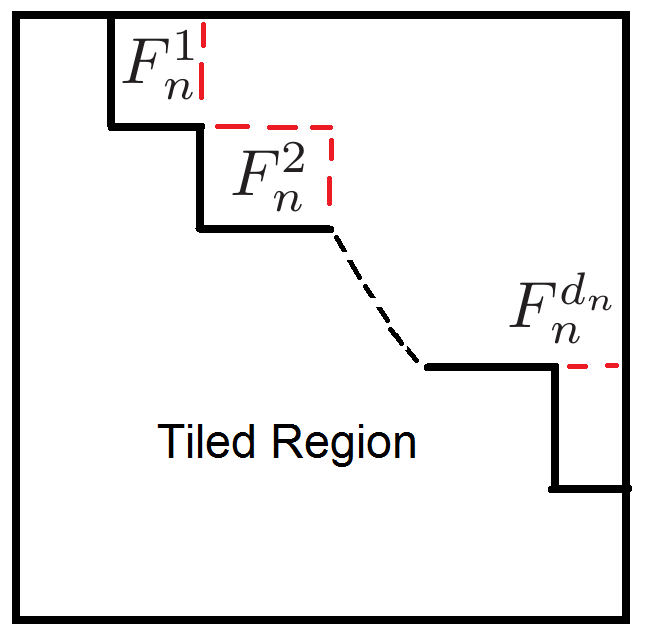
\includegraphics[width=0.8\linewidth]{Algorithm}
\captionof{figure}{Example Configuration}
\end{center}

\end{multicols}

%------------------------------------------------



}

%----------------------------------------------------------------------------------------
%	REFERENCES
%----------------------------------------------------------------------------------------

\headerbox{References}{name=references,column=2,span=2,above=bottom}{ % This block is as tall as the references block

\renewcommand{\section}[2]{\vskip 0.05em} % Get rid of the default "References" section title
\nocite{*} % Insert publications even if they are not cited in the poster

\bibliographystyle{unsrt}


\bibliography{Mentorship_Poster} % Use sample.bib as the bibliography file

}


%----------------------------------------------------------------------------------------
%	FUTURE INVESTIGATION
%----------------------------------------------------------------------------------------

\headerbox{$2$ by $1/2$ Rectangle}{name=futureresearch,column=0,span=2,above=bottom}{ % This block is as tall as the references block

\begin {center}
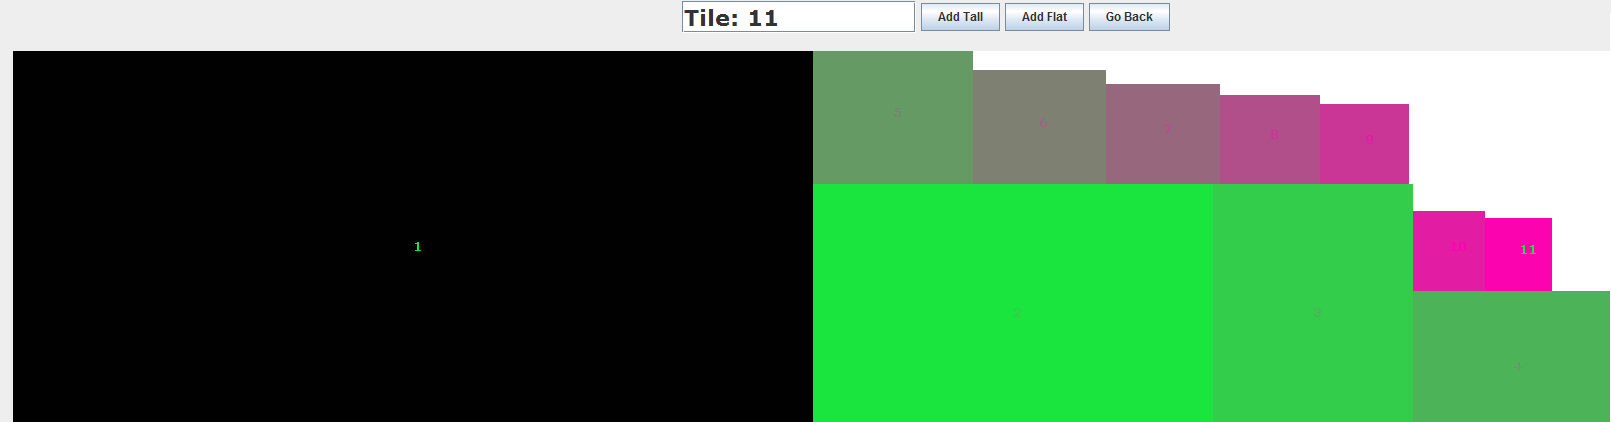
\includegraphics[width=0.8\linewidth]{Config_2}
\captionof{figure}{$2$ by$\frac{1}{2}$ - 11 Tiles}
\end{center}

}


%----------------------------------------------------------------------------------------
%	CONCLUSION
%----------------------------------------------------------------------------------------

\headerbox{Conclusion \& Results}{name=conclusion,column=2,span=2,row=0,below=algorithm}{

\begin{multicols}{2}


%------------------------------------------------

\begin{itemize}\compresslist
\item No configuration satisfying our hypothesis was found to exist
\item Simulated through nearly $40,000$ configurations witih depth first search through all positions and rotations for $T_k$ 
\item Surprisingly, \textbf{no} tiling with more than 12 tiles was found to be achievable
\item Other rectangles of area 1 ($\frac{a}{b}$ $\cdot$ $\frac {b}{a}$) were explored with similar results
\item A $\frac{4}{3}$ by $\frac {3}{4}$ was tiled with up to 14 tiles
\item A $2$ by $\frac {1}{2}$ was tiled with up to 11 tiles
\item An algorithm to tile the unit square should less conservative and use regions outside of the defined freespace
\end{itemize}
\begin{center}
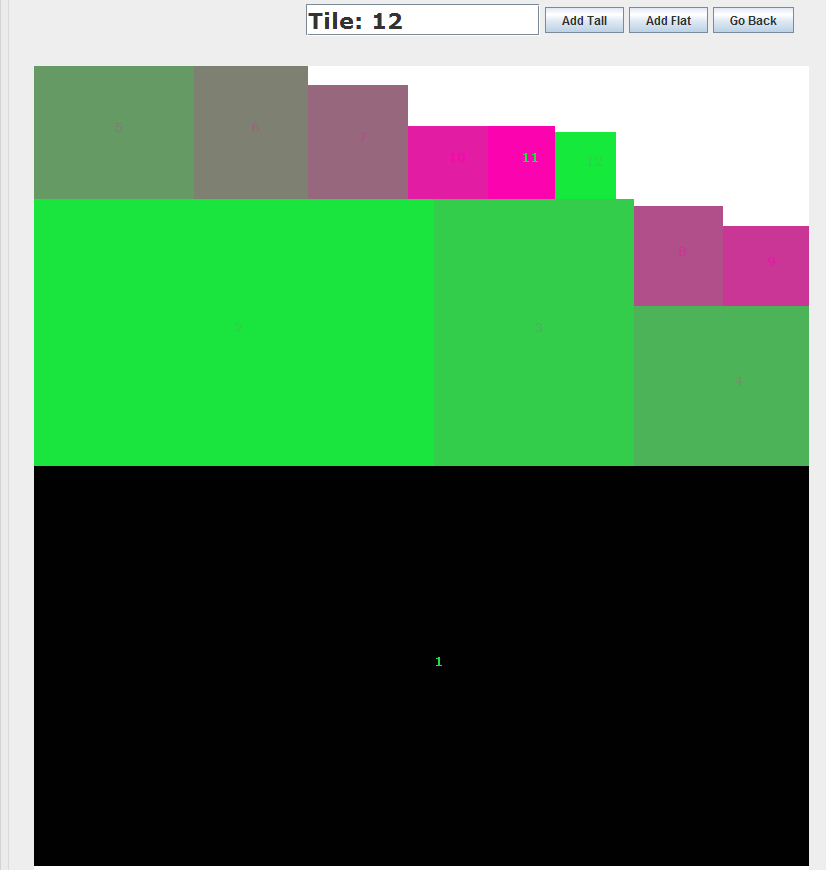
\includegraphics[width=0.8\linewidth]{Config_12A}
\captionof{figure}{Unit Square - 12 Tiles}
\end{center}

\end{multicols}
}

%----------------------------------------------------------------------------------------
%	APPROACH & HYPOTHESISt
%----------------------------------------------------------------------------------------

\headerbox{Hypothesis \& Approach }{name=approach,column=0,span=2,below=intro}{ % This block's bottom aligns with the bottom of the conclusion block

\textbf{Definition:}
\begin{itemize}\compresslist
\item\textit{Tile $T_k$} - The kth rectangle to be added, with dimensions $\frac{1}{k}$ by $\frac{1}{k+1}$ 
\item\textit{Free Space} - The region $T_0\setminus\bigcup_{i=1}^{n}T_i$. We further subdivide this into rectangles $F_n(1),F_n(2),\ldots,F_n(m_n)$ and denote those with boundary touching the tiled region by $F_n^1,F_n^2,\ldots,F_n^{d_n}$   
\end {itemize}

We looked for an algorithm that adds the tiles $T_1,T_2,\ldots$ in order. The following hypotheses are made and notation is  used in our approach:

\begin{itemize}\compresslist
\item The tiles are added parallel to the sides of $T_0$
\item For each $n\in\mathbb{N}$, the free space is connected and simply connected
\item The intersection of the tiled space with horizontal or vertical lines is connected
\end{itemize}

Observe that a tile placed inside a free tile will only decrease the perimeter if the tile touches the boundary of the unit tile.		

}


%----------------------------------------------------------------------------------------

\end{poster}

\end{document}